\lipsum[1-4]

\section{ZigBee}

ZigBee jest standardem transmisji bezprzewodowej zapewniający niskokosztową platformą
możliwą do zastosowania w elektronice użytkowej, automatyce domowej, wszelkiego rodzaju sensorach
(w~szczególności przemysłowych i~medycznych) jak również grach i~zabawkach.
Pierwsza specyfikacja opublikowana została w grudniu 2004 roku będąc ciągle aktualizowana,
z najnowszą jej wersją będącą datowaną na marzec 2017 roku~\cite{zigbee_alliance_zigbee_2017}.

Architektura ZigBee oparta została o IEEE 802.15.4. Definiuje ona fundamentalne zagadnienia:
\gls{PHY} i~\gls{MAC}. Warstwa fizyczna odpowiada za funkcjonowanie
radia, \gls{LQI}, transmisję danych i~odbiór pakietów poprzez łącze fizyczne. Definiuje dozwolone
częstotliwości działania, szerokości pasma, rodzaj modulacji i~dozwoloną przepustowość danych
wyrażonych w bitach na sekundę. Warstwa MAC odpowiada za komunikację w wyższych warstwach stosu.
Obejmuje to między innymi zarządzanie dostępem do kanałów, walidacja ramek danych, informację
zwrotną o~otrzymaniu i~przetworzeniu danych~\gls{ACK} oraz zapewnia odpowiednie
uchwyty celem umożliwienia wdrożenia mechanizmów zabezpieczeń.
Standard wprowadza również pojęcie topologii uwzględniając tym samym sposoby,
w~jakich można zorganizować sieć poszczególnych urządzeń. Definiowane są dwie
opcje połączeń: gwiazda, peer-to-peer. Topologia gwiazdy pozwala podłączenie wielu węzłów
uwzględniając fakt, iż komunikacja odbywa się za pośrednictwem koordynatora \gls{PAN},
będący tożsamy z \gls{FFD}. W~przypadku konfiguracji rówieśniczej, urządzenia mogą 
komunikować się dodatkowo między sobą, zapewniając możliwość ustanowienia innych struktur, m.in. 
Mesh. Standard wprowadza określenie \gls{RFD}, będące najczęściej urządzeniem o~prostej funkcjonalności 
niewymagającym dużych ilości danych do funkcjonowania, o~zredukowanej potrzebie na 
zasoby sprzętowe~\cite{ieee_p80215_working_group_ieee_nodate}.

\begin{figure}[!ht]
	\centering 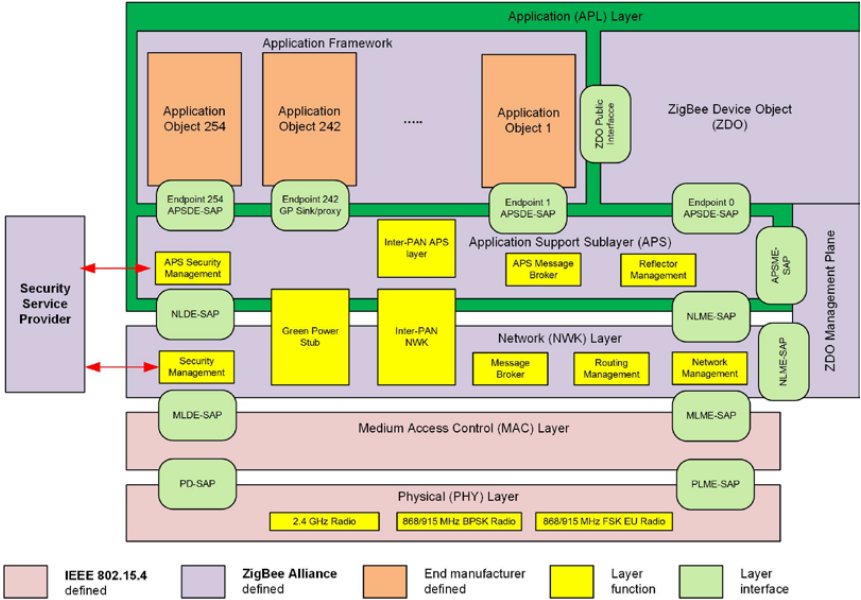
\includegraphics[width=0.99\linewidth]{zigbee_stack_architecture.png}
	\caption{Architektura stosu ZigBee. Źródło:~\cite{zigbee_alliance_zigbee_2017}}
	\label{rys:zigbee_stack_architecture}
\end{figure}

Specyfikacja ZigBee, opierając się na dokumentach IEEE 802.15.4, wykorzystuje częstotliwości
$868/915 MHz$ (w zależności od regionu Europa albo USA/Australia) oraz 2.4GHz~\cite{zigbee_alliance_zigbee_2017}.
Umożliwia tym samym transfer z przepustowością do 250~kbps~\cite{silicon_laboratories_ug10302_2021}.
Omawiany standard wprowadza swoje dodatkowe warstwy komunikacji do stosu: \gls{NWK} oraz~\gls{APL} --
Rysunek~\ref{rys:zigbee_stack_architecture}.
Warstwa aplikacji, będącą najwyższą w~hierarchi, składa się z wielu składowych. \gls{APS} odpowiada za
komunikację pomiędzy \gls{NWK} a~warstwami wyższymi. Oferuje między innymi parowanie urządzeń,
przekazywanie wiadomości, adresację, zajmuje się fragmentacją pakietów i~zapewnia niezawodny transport danych.
\gls{ZDO} w~głównej mierze odpowiada za wyszukiwanie urządzenia i~usług ZigBee~\cite{stmicroelectronics_an5506_2020, zigbee_alliance_zigbee_2017}.
Nadaje on również role urządzeniom sieci.

\begin{figure}[!ht]
	\centering 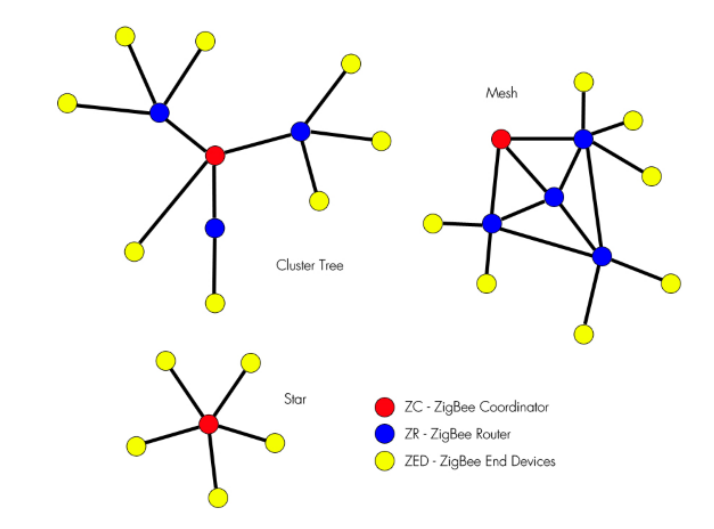
\includegraphics[width=0.618\linewidth]{zigbee_topologies_an5506.png}
	\caption{Topologie sieci ZigBee. Źródło:~\cite{stmicroelectronics_an5506_2020}}
	\label{rys:zigbee_topologies_an5506}
\end{figure}

ZigBee wprowadza trzy główne definicje ról urządzeń rejestrowanych do wewnątrz sieci:
\begin{itemize}
\item \gls{ZC} -- węzeł odpowiadający za utworzenie i~utrzymywanie scentralizowanej sieci, dobór wymaganych parametrów, dodawanie nowych węzłów.
\item \gls{ZR} -- węzeł odpowiadający za przekazywanie danych, który również może przyjąć rolę urządzenia końcowego. 
\item \gls{ZED} -- węzeł końcowy który odbiera i wysyła dane bez możliwości ich routowania.
\end{itemize}

Warstwa sieci umożliwia adaptację trzech rodzajów topologii: gwiazda, drzewo i mesh -- Rysunek~\ref{rys:zigbee_topologies_an5506}.
Typ gwiazdy kontrolowany jest przez jednego koordynatora. Topologia drzewa pozwala zastosować hierarchiczne
sposoby routingu pakietów. Typ mesh z kolei pozwala na pełną komunikację peer-to-peer między węzłami~\cite{zigbee_alliance_zigbee_2017}.
Zestawienie poszczególnych warstw z~modelem referencyjnym OSI znajduje się na Rysunku~\ref{rys:zigbee_osi_comparison_an5506}.

ZigBee umożliwia wykorzystanie następujących metod routingu. Metoda oparta o tablicę trasowania\footnote{z ang. \textit{Routing Table}}
zakłada, iż każdy z~węzłów posiada strukturę przechowującą adresy kolejnych, otaczających go węzłów. Raz wysłana wiadomość,
będzie korzystać z~tej informacji, by przesłać pakiet do miejsca docelowego. W~przypadku niepowodzenia, pierwotny węzeł otrzyma
błąd, by ewentualnie podjąć dalszą decyzję o~ponownym wyznaczeniu trasy. Standard przewiduje wysyłanie również pakietów
przy wykorzystaniu rozgłoszenia z możliwością wyboru roli danego urządzenia. Możliwy jest również multicast. Ostatnią
opcją trasowania jest metoda wiele-do-jednego (źródła)~\cite{silicon_laboratories_ug10302_2021}.

\begin{figure}[!ht]
	\centering 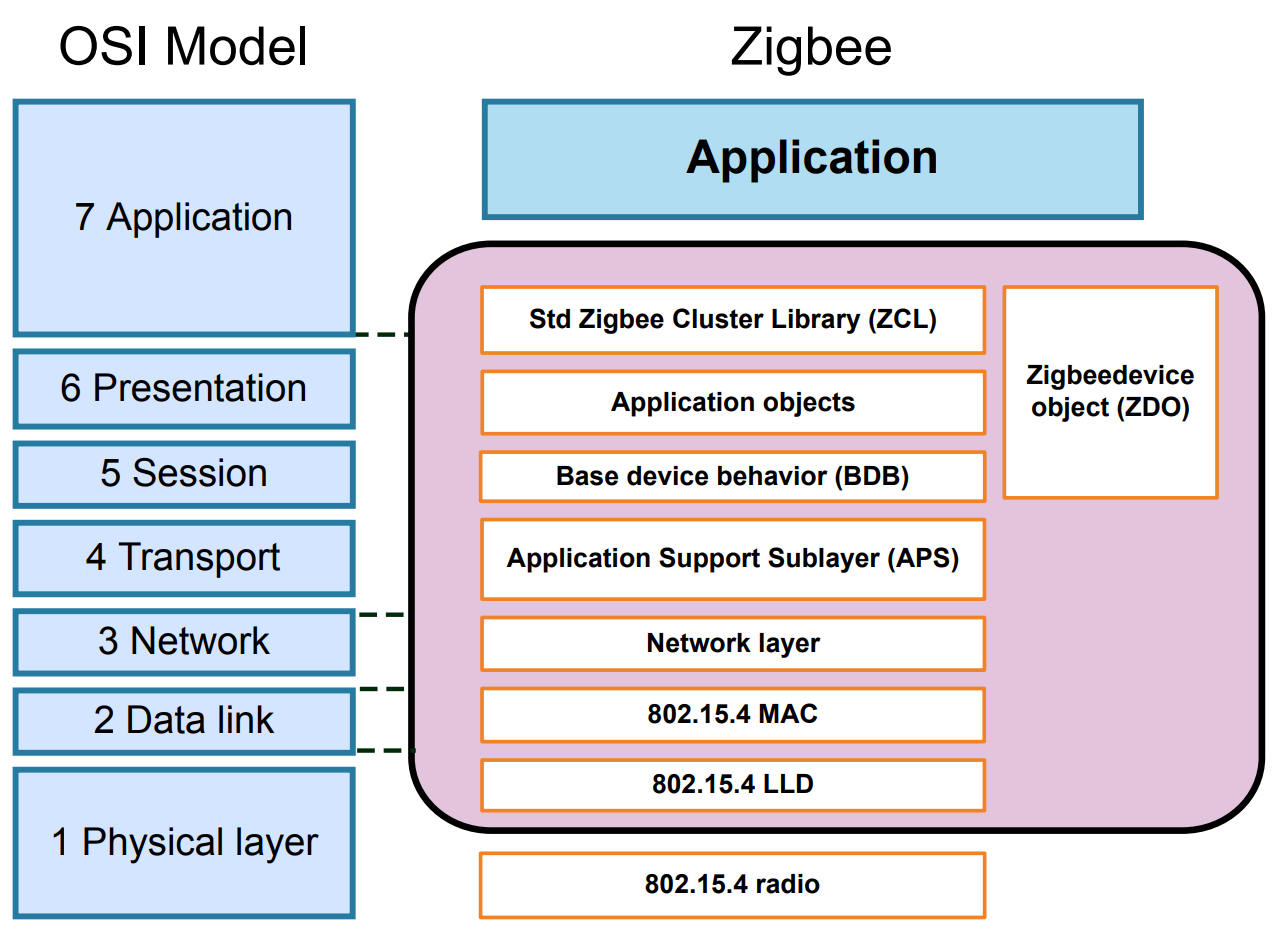
\includegraphics[width=0.618\linewidth]{zigbee_osi_comparison_an5506.png}
	\caption{Zestawienie warstw stosu ZigBee z modelem referencyjnym OSI. Źródło:~\cite{stmicroelectronics_an5506_2020}}
	\label{rys:zigbee_osi_comparison_an5506}
\end{figure}

ZigBee wprowadza termin \textit{profili}, będący kontraktem pomiędzy komunikatami wysyłanymi pomiędzy urządzeniami. Definiuje on
logiczną strukturę danych i zapewniając kompatybilność pomiędzy platformami różnych producentów. Cechą tą charakteryzują
się przede wszystkim profile publiczne zdefiniowane przez ZigBee Alliance. Poszczególni producenci mogą 
również opracować własnościowe, zamknięte struktury do tworzenia wewnętrznych sieci, gdzie kompatybilność pomiędzy
urządzeniami wielu producentów nie jest wymagana~\cite{zigbee_alliance_zigbee_2017, stmicroelectronics_an5506_2020, zigbee_alliance_zigbee_2017}.

\section{Thread}
Thread jest protokół to do zastosowań \gls{IoT} mający swe podstawy w standardzie IEEE 802.15.4.
Umożliwia on tworzenie rozwiązań o niskim zużyciu energii, przy jednoczesnej koncentracji na bezpieczeństwie opierając
adresację o powszechnie znany IPv6. Wybór IPv6 zapewnia płynną integrację z~powszechną infrastrukturą
i~Internetem włącznie. Rozwiązanie jest przez to elastyczne i~mniej podatne na starzenie się technologii.
Same natomiast produkty oparte o~Thread mogą być wdrożone na rynek szybciej dzięki powszechności
internetowych narzędzi deweloperskich. Pierwsza wersja specyfikacji została udostępniona
w 2014 roku i~pozostaje rozwijana do dziś~\cite{noauthor_thread_nodate}.

\begin{figure}[!ht]
	\centering 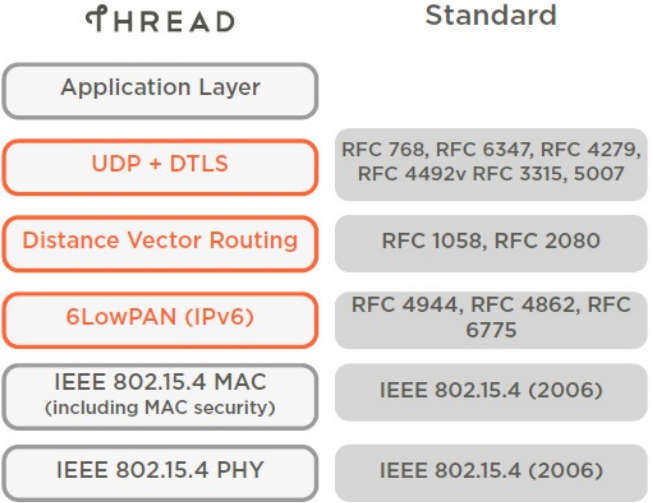
\includegraphics[width=0.618\linewidth]{thread_stack_overview_ug10311.png}
	\caption{Stos Thread i odpowiadające mu specyfikacje RFC/IEEE. Źródło:~\cite{silicon_laboratories_ug10311_2022}}
	\label{rys:thread_stack_overview_ug10311}
\end{figure}

Thread wykorzystuje standard IEEE 802.15.4. Transmisja danych odbywa się na częstotliwości $2.4GHz$ z przepustowością
do 250~kbps. Protokół jest zoptymalizowany do wykorzystywania dużej liczby węzłów wchodzących w skład sieci~\cite{silicon_laboratories_ug10311_2022}.
Celem organizacji sieci w~spójny zbiór fizycznych i~logicznych obiektów, standard wprowadza następującą nomenklaturę.
Rolą węzła typu router jest przekazywanie pakietów w sieci oraz nadzorowanie dostępu do sieci, podczas gdy radio
takiego urządzenia ciągle jest w aktywne. \gls{ED} jest urządzeniem przeważnie komunikującym się z~jednym
routerem będącym jego rodzicem, nie przekazuje pakietów dla innych sieci i~możliwością deaktywacji radia
celem ograniczenia zużycia energii. Dodatkowo, definiuje się następujące typy urządzeń:
\begin{itemize}
\item \gls{FTD} -- urządzenie posiadające ciągle włączone radio, mapujące adresację IPv6
	\begin{itemize}
	\item Router
	\item \gls{REED} -- urządzenie, które można wykorzystywać jako router
	\item \gls{FED} -- urządzenie, którego nie można wykorzystywać jako router
	\end{itemize}
\item \gls{MTD} urządzenie przekazujące komunikaty do rodzica.
	\begin{itemize}
	\item \gls{MED} -- urządzenie, którego radioodbiornik zawsze pozostaje włączony. Nie wymaga periodycznego
	pobierania wiadomości z urządzenia-rodzica
	\item \gls{SED} -- urządzenie wzbudzające radioodbiornik okazjonalnie celem pobrania wiadomości.
	\end{itemize}
\end{itemize}
Standard przewiduje dodatkowe typy jak Thread Leader, będący dynamicznie i automatycznie wybieranym węzłem
zarządzający pozostałymi Router'ami w sieci. Border Router (router brzegowy) służy za bramkę
konwertujący komunikaty przesyłane wewnątrz sieci Thread do sieci zewnętrznych takich jak Internet~\cite{noauthor_node_2022}.

\begin{figure}[!ht]
	\centering 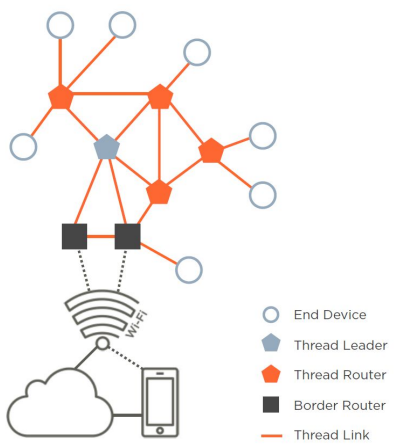
\includegraphics[width=0.618\linewidth]{thread_topology_devices_threadgroup.png}
	\caption{Podstawowa topologia sieci Thread wraz z urządzeniami. Źródło:~\cite{thread_group_thread_2020}}
	\label{rys:thread_topology_devices_threadgroup}
\end{figure}

Dane w sieci przesyłane są w oparciu o~standard \textit{6LoWPAN}\footnote{IPv6 Over Low Power Wireless Personal Networks}.
Protokół ten został zoptymalizowany w ten sposób, by wysyłać maksymalną możliwą ilość danych z użyciem jednego
pakietu celem minimalizacji fragmentacji pakietów, redukując tym samym narzut na CPU i~zużycie energii.
Thread umożliwia stosowanie również protokołów znanych z sieci opartych o model TCP/IP. Tak więc
standard ten obsługuje m.in. \gls{ICMP}, \gls{UDP}, \gls{TCP}. Topologia tym samym również zależy od ilości
węzłów typu router, tworząc albo sieć gwiazdy, albo mesh. Thread obsługuje do 32-óch routerów, gdzie każdy
z~nich może obsłużyć do 511 \gls{ED}. Routing odbywa się na zasadach znanych z~\gls{IP}
wykorzystując w tym celu protokół zbliżony do \gls{RIP}, będący zoptymalizowany do wymagań
IoT pod względem zużycia energii~\cite{silicon_laboratories_ug10311_2022}.

\begin{figure}[!ht]
	\centering 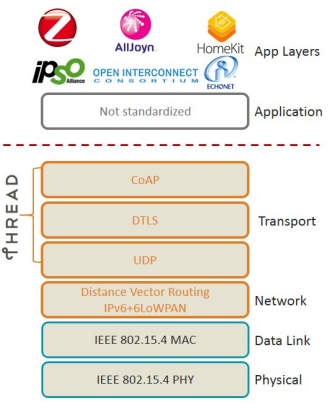
\includegraphics[width=0.618\linewidth]{thread_iso_comparison_ug10311.png}
	\caption{Thread w zestawieniu z modelem OSI. Źródło:~\cite{silicon_laboratories_ug10311_2022}}
	\label{rys:thread_iso_comparison_ug10311}
\end{figure}

Thread będący otwartym standardem może zostać wdrożony przez producenta samodzielnie bądź wybrać stos otwartoźródłowy --~\ref{rys:thread_iso_comparison_ug10311}.
Jednym z takich stosów jest OpenThread\footnote{\url{https://openthread.io/}} będący opracowany przez firmę Google.

Co warto dodać, Thread nie definiuje formatu danych jaki jest wysyłany pomiędzy węzłami. Innymi słowy,
warstwa aplikacji jest nieustandaryzowana~\cite{silicon_laboratories_ug10311_2022}. Obecnie trwają
prace nad opracowaniem wspólnego i~wolnościowego interfejsu. Jednym z takich projektów jest \textit{Matter}\footnote{\url{https://csa-iot.org/all-solutions/matter/}}.

\section{Bluetooth Low Energy}
\lipsum[1-8]

\section{Porównanie przedstawionych standardów} % jako podroździał
% historia jako delikatny wstęp
\url{https://www.silabs.com/documents/public/application-notes/an1142-mesh-network-performance-comparison.pdf}
\url{https://www.silabs.com/wireless/matter}
\lipsum[1-15]


% 1. Krótki rys historyczny standardu
% 2. Opis stosu + jakiś obrazek
% 2.1. Częstotliwości na których pracuej standard
% 3. Topologia, rodzaje węzłów
